\section{Model matematyczny}
Przyjmując zerowy kąt wychylenia $\phi$ w górnym położeniu równowagi wahadła założono, że wartości rosną w kierunku matematycznie ujemnym (zgodnie z ruchem wskazówek zegara).  
\begin{figure}[H]
\centering
\label{fig:www}
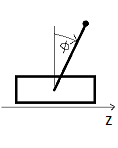
\includegraphics[width=3cm]{obrazy/wozek2.png}
\caption{Schemat wahadła na wózku}
\end{figure}
Na rysunku \ref{fig:www} zaznaczono kierunki mierzenia kąta wychylenia wahadła oraz położenia wózka.
\subsection{Wyprowadzenie modelu}
Rozważając wahadło oddzielnie od wózka wprowadzono siły reakcji więzów $H(t)$ oraz $V(t)$. Pierwsza z nich działa w kierunku poziomym wzdłuż szyny, natomiast druga prostopadle do niej.
\begin{equation}
\label{eq:fiz}
\begin{aligned}
&m\dfrac{d^2}{dt^2}[z(t)+l\sin \phi(t)] = H(t)\\
&m\dfrac{d^2}{dt^2}[l\cos \phi(t)] = V(t)-mg\\
&J_{sm}\dfrac{d^2\phi(t)}{dt^2} = lV(t)\sin \phi(t)-lH(t)\cos \phi(t)
\end{aligned}
\end{equation}
Równania \ref{eq:fiz} są wynikiem zastosowania drugiej zasady dynamiki Newtona dla kolejno: sił działających na wahadło w poziomie, sił pionowych oraz momentów obrotowych względem środka ciężkości wahadła. Symbol $m$ oznacza całkowitą masę wahadła.

Po przekształceniach układu \ref{eq:fiz}, mając na uwadze równanie dynamiki wózka \ref{eq:zz} otrzymano równanie:
\begin{equation}
\label{eq:rowNonLin}
\ddot{\phi}=\dfrac{mgl}{J_{sm}+ml^2}\sin\phi+\dfrac{mlc_1}{J_{sm}+ml^2}\dot{z}\cos\phi-\dfrac{mlc_2}{J_{sm}+ml^2}u\cos\phi
\end{equation}
W celu sprawdzenia poprawności wyprowadzonego modelu wygenerowano przykładowe sterowanie oraz porównano zarejestrowane przebiegi z modelowymi:
\begin{figure}[H]
\centering
\label{fig:poW}
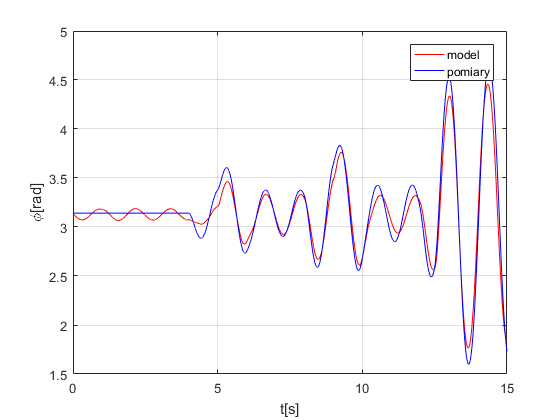
\includegraphics[width=12cm]{obrazy/rad.png}
\caption{Położenie kątowe wahadła}
\end{figure}
\begin{figure}[H]
\centering
\label{fig:prW}
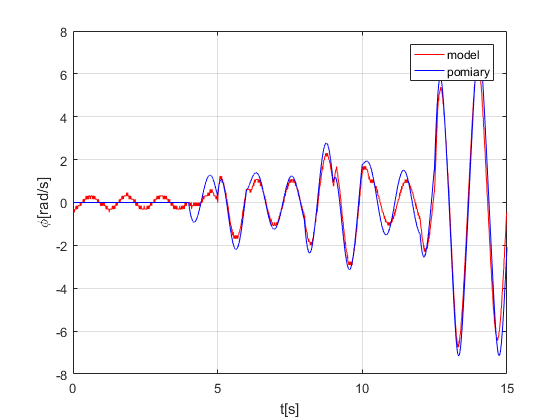
\includegraphics[width=12cm]{obrazy/radPerSec.png}
\caption{Prędkość kątowa wahadła}
\end{figure}
\subsection{Równania stanu}
Zidentyfikowany model dynamiki wózka oraz dynamiki wahadła pozwala na zapis równań stanu systemu w standardowej formie $\dot{\textbf{x}}=f(\textbf{x},u)$. Przyjmując następujące zmienne stanu:
\begin{equation}
\label{eq:rStan}
\begin{aligned}
x_{1} = \phi \\
x_{2} = \dot{\phi} \\
x_{3} = z\\
x_{4} = \dot{z}
\end{aligned}
\end{equation}
nieliniowe równania stanu przyjmują postać:
\begin{equation}
\label{eq:rStan}
\begin{aligned}
&\dot{x_{1}} = x_2 \\
&\dot{x_{2}} = \dfrac{mgl}{J_{sm}+ml^2}\sin x_1+\dfrac{mlc_1}{J_{sm}+ml^2}x_4\cos x_1-\dfrac{mlc_2}{J_{sm}+ml^2}u\cos x_1 \\
&\dot{x_{3}} = x_4\\
&\dot{x_{4}} = -c_1x_4+c_2u
\end{aligned}
\end{equation}
